\documentclass[
]{jss}

%% recommended packages
\usepackage{orcidlink,thumbpdf,lmodern}

\usepackage[utf8]{inputenc}

\author{
Søren B. Vilsen\\Department of Mathematical Sciences, Aalborg University
}
\title{Random weight neural networks in \proglang{R}: The \pkg{RWNN}
package}

\Plainauthor{Søren B. Vilsen}
\Plaintitle{Random weight neural networks in R: The RWNN package}
\Shorttitle{\pkg{RWNN}: Random Weight Neural Networks}


\Abstract{
This paper serves as an introduction to the \pkg{RWNN} package. The
\pkg{RWNN} package implements random weight neural networks. The methods
are implemented using a combination of \proglang{R} and \proglang{C++}
offsetting the heavier computation and estimation to \proglang{C++}
through the \pkg{Rcpp} and \pkg{RcppArmadillo} packages. While
implementations of random weight neural networks exist other
\proglang{R} packages, these focus on the simplest possible variant of
the random weight neural network and cover only very specialised use
cases of these networks. Besides a general purpose implementation of
random weight neural networks, the \pkg{RWNN} package also includes
common variants such as deep RWNN and sparse RWNN, as well as ensemble
methods using random weight neural networks as the base learner.
}

\Keywords{random weight neural networks, regularisation, ensemble
learning, Bayesian
computation, \proglang{R}, \pkg{Rcpp}, \pkg{RcppArmadillo}}
\Plainkeywords{random weight neural networks, regularisation, ensemble
learning, Bayesian computation, R, Rcpp, RcppArmadillo}

%% publication information
%% \Volume{50}
%% \Issue{9}
%% \Month{June}
%% \Year{2012}
%% \Submitdate{}
%% \Acceptdate{2012-06-04}

\Address{
    Søren B. Vilsen\\
    Department of Mathematical Sciences, Aalborg University\\
    Skjernvej 4A,\\
9220 Aalborg East\\
  E-mail: \email{svilsen@math.aau.dk}\\
  URL: people.math.aau.dk/\textasciitilde svilsen\\~\\
  }


% tightlist command for lists without linebreak
\providecommand{\tightlist}{%
  \setlength{\itemsep}{0pt}\setlength{\parskip}{0pt}}



%% preamble

\usepackage[utf8]{inputenc}
\usepackage[british]{babel}

\usepackage{amsmath, amssymb, bm}





\begin{document}



\hypertarget{introduction}{%
\section{Introduction}\label{introduction}}

Neural networks, and variants thereof, have seen a massive increase in
popularity in recent years. This has largely been due to the flexibility
of the neural network architecture, and their accuracy when applied to
highly non-linear problems. However, due to the highly non-linear nature
of the neural network architecture, estimating the weights of these
networks using gradient based optimisation (i.e.~back-propagation), can
be slow and does not guarantee a globally optimal solution. In order to
combat these problems, various simplifications of the feed forward
neural network (FFNN) architecture have been proposed, including random
weight neural networks (RWNNs). They were first introduced in the early
1990's under the name random vector functional links (RVFL)
\citep[\citet{Pao1994}]{Schmidt1992}, and a simplified version was
re-discovered under the name extreme learning machines (ELM)
\citep{Huang2006} in the mid 2000's. The general idea of RWNNs is to
keep the randomly assigned weights of the network between the
input-layer and the last hidden-layer fixed, and focus on estimating the
weights between the last hidden-layer and the output-layer. In the case
of regression, this simplification makes estimating the output weights
of a RWNN equivalent to estimating the weights of a (regularised) linear
model. Theoretically RWNNs show similar universal approximation
properties as their FFNN counterparts, i.e.~as the number of neurons
tends towards infinity the RWNN should be able to approximate any
function arbitrarily well (placing only loose assumptions on the
activation function). However, practically the number of neurons needed
for this approximation to be acceptable may not be feasible for a
particular application. Therefore, extensions of RWNNs have been
proposed limiting the number of neurons in favour of deeper
architecture, as seen in deep RWNN \citep{Henriquez2018} and ensemble
deep RWNN \citep{Shi2021}, or in favour of sparse unsupervised
pre-training of the weights, like sparse RWNN \citep{Zhang2019}.

Implementations of RWNNs already exist in \proglang{R} through the
packages \pkg{nnfor} \citep{nnfor} and \pkg{elmNNRcpp}
\citep{elmNNRcpp}, both focusing on the simpler ELM architecture. Both
implementations allow for a varying number of neurons in the
hidden-layer, as well as the specification of the activation function,
but are limited to a single hidden-layer with no functional link between
the input- and output-layers. The \pkg{nnfor} package was designed for
using ELMs to handle time-series data and allows for forecasting at
different temporal frequencies using the \pkg{thief} package.
Furthermore, it allows for estimation of the output-weights using
Moore-Penrose inversion, \(\ell_1\)-regularisation, and
\(\ell_2\)-regularisation. The \pkg{elmNNRcpp} package is the successor
to \pkg{elmNN} package \citep{elmNN} re-implemented in \proglang{C++}
through \pkg{Rcpp} and \pkg{RcppArmadillo} \citep[\citet{RcppA}]{Rcpp}.
The package is a standard implementation of the ELM architecture for
both regression and classification. The package allows the user to
specify the leakage of the implemented relu activation function, as well
as the tolerance of the Moore-Penrose inversion used to estimate the
output-weights.

\pkg{RWNN} is a general purpose implementation of RWNNs in \proglang{R}
\citep{R} focusing on regression problems. The \pkg{RWNN} package allows
the user to create an RWNN of any depth, set the number of neurons and
activation functions in each layer, choose the sampling distribution of
the randomly assigned weights, and choose whether the output weights
should be estimated by either Moore-Penrose inversion,
\(\ell_1\)-regularisation, or \(\ell_2\)-regularisation. The RWNN is
implemented in C++ through \pkg{Rcpp} and \pkg{RcppArmadillo}, and along
with the standard RWNN implementation the following variants have also
been included:

\begin{itemize}
\tightlist
\item
  \textbf{ELM} (extreme learning machine) \citep{Huang2006}: A
  simplified version of an RWNN without a link between the input and
  output layer.
\item
  \textbf{deep RWNN} \citep{Henriquez2018}: An RWNN with multiple hidden
  layers, where the output of each hidden-layer is included as features
  in the model.
\item
  \textbf{sparse RWNN} \citep{Zhang2019}: Applies sparse auto-encoder
  (\(\ell_1\) regularised) pre-training to reduce the number non-zero
  weights between the input and the hidden layer (the implementation
  generalises this concept to allow for both \(\ell_1\) and \(\ell_2\)
  regularisation).
\item
  \textbf{ensemble deep RWNN} \citep{Shi2021}: An extension of deep
  RWNNs using the output of each hidden layer to create separate RWNNs.
  These RWNNs are then used to create an ensemble prediction of the
  target.
\end{itemize}

Furthermore, the \pkg{RWNN} package also includes general
implementations of the following ensemble methods (using RWNNs as base
learners):

\begin{itemize}
\tightlist
\item
  \textbf{Stacking}: Stack multiple randomly generated RWNN's, and
  estimate their contribution to the weighted ensemble prediction using
  \(k\)-fold cross-validation.
\item
  \textbf{Bagging} \citep{Xin2021}: Bootstrap aggregation of RWNN's
  creates a number of bootstrap samples, sampled with replacement from
  the training-set. Furthermore, as in random forest, instead of using
  all features when training each RWNN, a subset of the features can be
  chosen at random.
\item
  \textbf{Boosting}: Gradient boosting creates a series of RWNN's, where
  an element, \(k\), of the series is trained on the residual of the
  previous \((k - 1)\) RWNN's. It further allows for manipulation of the
  learning rate used to improve the generalisation of the boosted model.
  Lastly, like the implemented bagging method, the number of features
  used in each iteration can be chosen at random (also called stochastic
  gradient boosting).
\end{itemize}

Lastly, the \pkg{RWNN} package also includes a simple method for grid
based hyperparameter optimisation, where \(k\)-fold cross-validation is
applied to training-set to find the hyperparameters yielding the
smallest cross-validation error on a supplied grid.

The remainder of the paper is structured as follows: Section \ref{RWNN}
introduces the general idea of RWNNs, this is followed by the method of
estimating the output weights, and an outline of each of the implemented
RWNN variants. The utility of the \pkg{RWNN} package is shown in Section
\ref{EX} applying different RWNN variants to a series of examples.
Lastly, a conclusion is found in Section \ref{CON}.

\hypertarget{RWNN}{%
\section{Random Weight Neural Networks}\label{RWNN}}

The general structure of an RWNN with a single hidden-layer can be seen
in Figure \ref{fig:rwnn}. The RWNN is a simplification of a simple FFNN,
where the weights between the input-layer and the hidden-layer are kept
fixed after the randomly initialisation of the network. That is, the
weights between the last hidden-layer and the output-layer are the only
weights estimated during the training process. Furthermore, an RWNN may
include a direct (also called functional) link between the features and
the output, shown as dashed lines in Figure \ref{fig:rwnn}. When these
links are active, the output can be seen as a concatenation of the last
hidden-layer and the input-layer (i.e.~a concatenation of the both the
original and random non-linear transformation of the features). Using
this simplification, the estimation of the output-weights simplifies
greatly if the activation between the concatenated layer and the output
is linear (i.e.~the identity function), as estimating of the
output-weights becomes equivalent to estimating the weights in a
(regularised) multiple linear regression.

\begin{CodeChunk}
\begin{figure}

{\centering 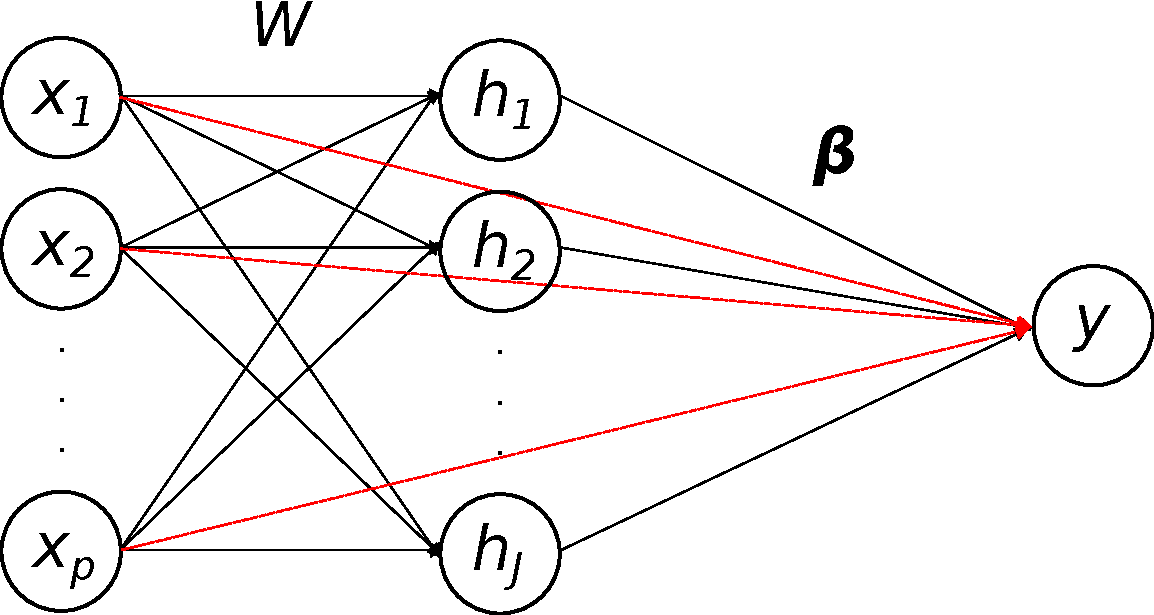
\includegraphics[width=0.6\linewidth]{./Figures/RWNN} 

}

\caption[Graph representation of a random weight neural network (RWNN) with funcitonal link between the input and the output layer]{Graph representation of a random weight neural network (RWNN) with funcitonal link between the input and the output layer.}\label{fig:rwnn}
\end{figure}
\end{CodeChunk}

Given a sample of \(N\) observations,
\(\mathcal D = \{(\boldsymbol x_n, y_n)\}_{n = 1}^N\), where
\(\boldsymbol x_n\) is \(p\) dimensional vector of features and \(y_n\)
is the output of observation \(n\), then the output of the \(j\)'th
neuron of the hidden layer: \begin{equation}
h_{nj} = f\left(\sum_{i = 1}^p w_{ij} x_{ni} + w_{0}\right), \label{eq:hidden}
\end{equation} \(f\) is the activation function, \(w_0\) is the bias,
and \(w_{ij}\) is the weight between the \(i\)'th feature and the
\(j\)'th neuron in \(n\)'th observation. If the hidden-layer contains
\(J\) neurons the vector, the vector of transformed features of the
hidden layer, denoted \(\boldsymbol h_{n}\), simplifying the notation of
Eq. \eqref{eq:hidden} to: \begin{equation}
\boldsymbol h_n = \boldsymbol f\left(W \boldsymbol{x}_n + w_0 \boldsymbol{1}_{J}\right),
\end{equation} where \(\boldsymbol{1}_{J}\) is a vector of one's of
dimension \(J\).

Let \(\boldsymbol d_n = [\boldsymbol h_n \; \boldsymbol x_n]^T\) be a
stacked vector of the features transformed by the hidden-layer, and
original features. Furthermore, assuming the activation in the
output-layer is linear, then the predicted response of the \(n\)'th
observation is: \begin{equation}
\hat{y}_n = \boldsymbol d^T_n \boldsymbol \beta.
\end{equation}

Given a concatenated matrix of features, \(D\), (i.e.~a matrix whose
\(n\)'th row contains \(\boldsymbol d_n\)) and \(\boldsymbol y\) be a
vector containing the output, the output-weights \(\boldsymbol \beta\)
can be found by minimising sum-of-squared errors (SSE): \begin{equation}
\hat{\boldsymbol{\beta}} = \underset{\boldsymbol{\beta}}{\text{argmin}} \Big\{ || \boldsymbol{y} - D\boldsymbol{\beta}||_2^2\Big\}. \label{eq:ssq}
\end{equation}

When \(N > p + J\), the solution to this system of equations can be
found by the normal equation: \begin{equation}
\hat{\boldsymbol{\beta}}^{(ols)} = (D^T D)^{-1}D^T\boldsymbol{y}. \label{eq:ols}
\end{equation}

However, in many application the number of concatenated features
(i.e.~the number of columns of \(D\)) is much bigger than the number of
observations, i.e.~\((p + J) >> N\). When this is the case, the two most
common approaches to estimating the parameters are the Moore-Penrose
pseudoinverse and regularisation.

When using Moore-Penrose pseudoinverse
\citep[\citet{PenroseInv}]{BjerhammarInv}, \(D^+\), the solution to the
optimisation problem is simply: \begin{equation}
\hat{\boldsymbol \beta}^{(p)} = D^+ \boldsymbol y.
\end{equation}

When regularisation is introduced the SSE, seen in Eq.~\eqref{eq:ssq},
is penalised by the size of the output-weights. The penalisation is
usually performed using \(\ell_1\) or \(\ell_2\) norm, creating the
following optimisation problem: \begin{equation}
\hat{\boldsymbol{\beta}} = \underset{\boldsymbol{\beta}}{\text{argmin}} \Big\{ || \boldsymbol{y} - D\boldsymbol{\beta}||_2^2  + \lambda||\boldsymbol{\beta}||_q^q \Big\}, \label{eq:rsse}
\end{equation} where \(q \in \{1, 2\}\) and \(\lambda\) is a
penalisation constant. The penalisation constant should be chosen such
that it minimises the out-of-sample error (using e.g.~\(k\)-fold
cross-validation during training process).

If \(q = 1\), the optimisation problem in Eq. \eqref{eq:rsse} is
equivalent to lasso regression \citep[\citet{TibLasso}]{SanLasso}.
Unlike ridge-regression it is not possible to find a closed form
solution of the lasso estimated output-weights,
\(\hat{\boldsymbol{\beta}}^{(lasso)}\), however, they can be found by
using coordinate descent \citep{CoordLasso}.

If \(q = 2\), the optimisation problem in Eq. \eqref{eq:rsse} is
equivalent to ridge-regression using the concatenated features, instead
of the input features, and the solution can be found as
\citep{ridgeReg}: \begin{equation}
\hat{\boldsymbol \beta}^{(ridge)} = \left(D^TD + \lambda I_{p + J}\right)^{-1}D^T\boldsymbol y,
\end{equation} where \(I_{p+J}\) is the identity matrix of size \(p+J\).

\textbf{NB:} Extreme learning machine's (ELM's) are effectively RWNN's
without the functional link and can, therefore, be trained using exactly
the same set of equations setting \(\boldsymbol d_n = \boldsymbol h_n\).

\hypertarget{deep-rwnn}{%
\subsection{Deep RWNN}\label{deep-rwnn}}

\begin{equation}
h_{nj}^{(k)} = f^{(k)}\left(\sum_{i = 1}^p w^{(k)}_{ij} h_{ni}^{(k - 1)} + w^{(k)}_{0}\right), \label{eq:hidden}
\end{equation} for \(k = 1, ..., K\), where \(h_{ni}^{(0)}\) is feature
\(x_{ni}\), \(f^{(k)}\) is the activation function, \(w^{(k)}_0\) is the
bias, and \(w^{(k)}_{ij}\) is the weight between the \(i\)'th feature
and the \(j\)'th neuron in the \(k\)'th layer. If the hidden-layer
contains \(J^{(k)}\) neurons the vector, the vector of transformed
features of the \(k\)'th layer is denoted \(\boldsymbol h^{(k)}_{n}\)
simplifying the notation of Eq. \eqref{eq:hidden} to: \begin{equation}
\boldsymbol h^{(k)} = \boldsymbol f^{(k)}\left(W^{(k)} \boldsymbol{h}^{(k)} + w^{(k)}_0 \boldsymbol{1}\right),
\end{equation} where \(\boldsymbol{1}\) is a vector of one's of
dimension \(J^{k}\).

Let \(\boldsymbol d_n = [\boldsymbol h^{(K)}_n \; \boldsymbol x_n]^T\)
be a stacked vector of the features transformed by the \(K\)
hidden-layers, and original features. Furthermore, assuming the
activation in the output-layer is linear, then the predicted response of
the \(n\)'th observation is: \begin{equation}
\hat{y}_n = \boldsymbol d^T_n \boldsymbol \beta
\end{equation}

\hypertarget{sparse-rwnn}{%
\subsection{Sparse RWNN}\label{sparse-rwnn}}

\hypertarget{ensemble-methods}{%
\subsection{Ensemble methods}\label{ensemble-methods}}

\hypertarget{stacking}{%
\subsubsection{Stacking}\label{stacking}}

\hypertarget{bagging}{%
\subsubsection{Bagging}\label{bagging}}

\hypertarget{boosting}{%
\subsubsection{Boosting}\label{boosting}}

\hypertarget{ensemble-deep-rwnn}{%
\subsection{Ensemble Deep RWNN}\label{ensemble-deep-rwnn}}

\hypertarget{EX}{%
\section{Examples}\label{EX}}

\hypertarget{CON}{%
\section{Conclusions}\label{CON}}

\renewcommand\refname{References}
\bibliography{literature.bib}



\end{document}
